\documentclass{beamer}

\usepackage[utf8]{inputenc}
\usepackage{hyperref}

\usetheme{Berkeley}
\beamertemplatenavigationsymbolsempty
\setbeamertemplate{headline}{}
 
\title{Erfassen von Daten in FoodChain-Lab 2}
\date{}
 
\begin{document}
\maketitle

\section{ }

\subsection{Aufgaben}
\begin{frame}
	\begin{itemize}
		\item
	\end{itemize}
\end{frame}
 
\subsection{1}
\begin{frame}
	\begin{center}
  		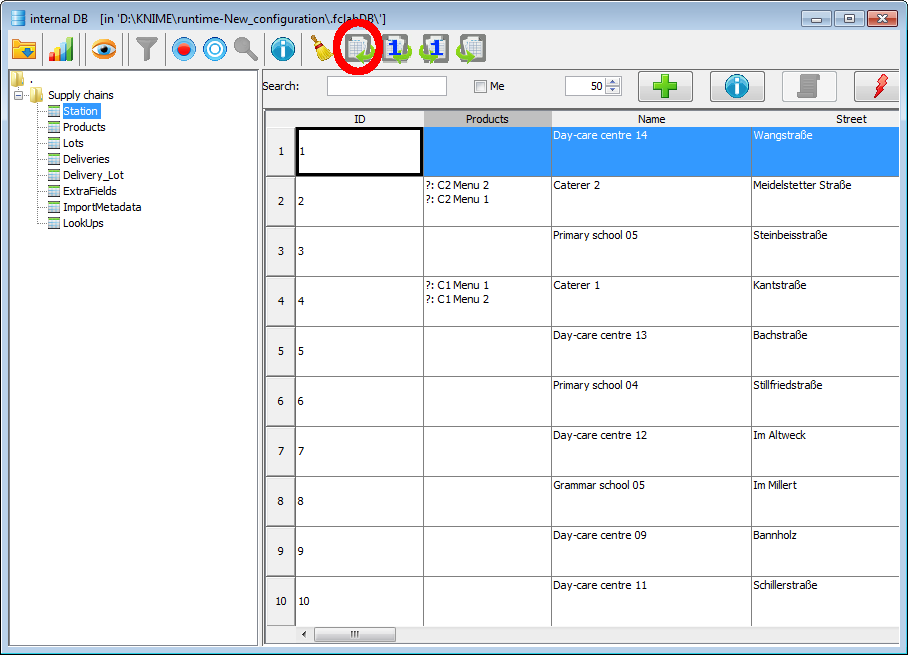
\includegraphics[height=0.6\textheight]{1.png}
	\end{center}
	\begin{itemize}
		\item Wählen Sie \textbf{Food-Lab $>$ Open DB Gui...} in der Menüleiste um das Datenbank-Fenster zu öffnen.
	\end{itemize}
\end{frame}

\end{document}